% Preview wrapper only: compiles shift_subsection.tex on its own. Not part of the paper.
% The \label definitions below stand in for the paper's own labels so that the references resolve.
\documentclass[10pt]{article}
\usepackage[letterpaper,margin=1.1in]{geometry}
\usepackage{amsmath,amssymb,graphicx,booktabs,array}
\usepackage[hidelinks]{hyperref}
\setlength{\parindent}{1em}
\begin{document}
\makeatletter
\def\@currentlabel{7}\label{tab:mcar}
\def\@currentlabel{3}\label{tab:hyperparams}
\def\@currentlabel{4.1.4}\label{sec:baselines}
\def\@currentlabel{2}\label{fig:performance}
\makeatother
\renewcommand{\cite}[1]{[ref]}
\setcounter{section}{4}
\setcounter{subsection}{3}
\setcounter{table}{9}
\setcounter{figure}{4}
% Subsection for the journal extension: frozen-model evaluation under missingness shift.
% Place after "Results on Complete Datasets" (it reuses that section's datasets and its 20% MCAR setting).
% Every number below is produced by telo_tabular.shift_report from runs_shift/; the table by telo_tabular.shift_table;
% the figures by telo_tabular.make_figures --datasets glass wdbc pima mushroom.
% In a two-column (sigconf) layout change figure/table to figure*/table*.

\subsection{Robustness to Missingness Shift at Test Time}
\label{sec:shift}

In all previous experiments the training and test partitions share the same missingness mechanism and rate. In practice
this is rarely guaranteed: a sensor may fail after deployment, or a field that was usually recorded may stop being
collected. Since 3C-EA evolves its activation function under one particular missingness regime, a natural question is
whether the resulting model remains reliable when that regime changes, or whether the evolved function is tied to the
conditions it was evolved under.

\subsubsection{Protocol}
We follow the setting of Table~\ref{tab:mcar}: 20\% MCAR missingness is injected into the training, validation and
test partitions, the activation function is evolved, and the selected function is retrained as described in
\S\ref{sec:baselines}. The model is then \emph{frozen}. Nothing is re-estimated at test time: the network weights, the
evolved function, the training means used for imputation, and the feature-wise confidence values, which are computed
from the training missing rates, all stay fixed. The same test records are then masked again under thirteen
conditions, the matched one and twelve shifted ones: MCAR at rates from 0\% (no injected missingness) to 60\%, and three structured mechanisms at 20\% and
40\%. In the \emph{grouped} mechanism each record loses a block of mutually correlated features, namely a randomly
chosen feature together with the features most correlated with it in the training data, which imitates the failure of
a group of related measurements. MAR and MNAR masks follow the rules of the previous section (for MAR, entries are
removed with a probability that depends on whether the first feature exceeds its median; for MNAR, with a higher
probability when the value itself lies outside the interquartile range), with the thresholds estimated on the training
partition. For the structured
mechanisms the stated rate is nominal; the realised fraction of missing entries lies between 0.14 and 0.25 for the
20\% conditions and between 0.27 and 0.49 for the 40\% conditions, depending on the dataset. The four fixed
activations are trained and evaluated in exactly the same way, with the same partitions, masks and random seeds, so
every comparison is paired by run.

The matched condition, in which the test data also contain 20\% MCAR missingness, repeats the setting of
Table~\ref{tab:mcar} with the reduced search budget given below and serves only as the reference for the twelve
shifted conditions.

We report Glass, WDBC, PIMA and Mushroom. Glass, WDBC and PIMA use a population of 70 and 15 generations with 10
independent runs; Mushroom uses a population of 100 and 10 generations with 20 runs. The remaining GP settings are
those of Table~\ref{tab:hyperparams}. For each condition, 3C-EA is compared with the fixed activation that has the
highest mean accuracy under that condition. Because the best baseline is selected after the results are known, this
comparison favours the baselines. Significance is assessed with a two-sided Wilcoxon signed-rank
test~\cite{derrac2011practical} on the paired per-run accuracies, without correction for multiple comparisons.

\begin{figure}[t]
\centering
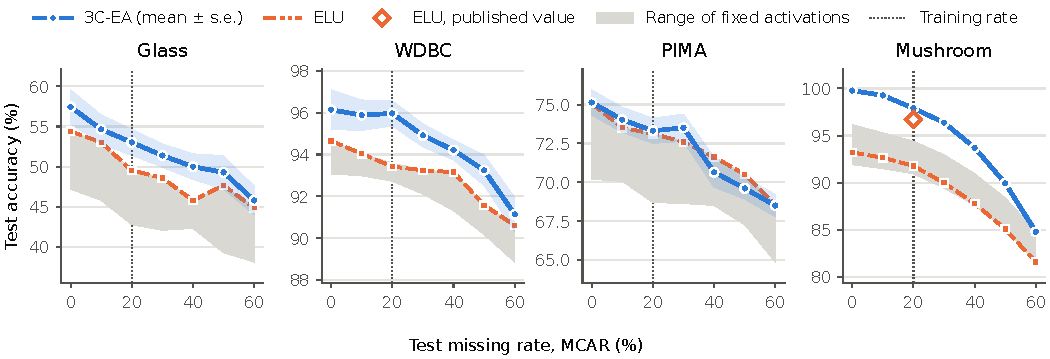
\includegraphics[width=\linewidth]{figures/fig_shift_curves.pdf}
\caption{Test accuracy when the test missing rate differs from the training rate. All models are trained with 20\%
MCAR missingness (dotted line) and evaluated without retraining at MCAR rates from 0\% to 60\%. The solid line is
3C-EA (mean over runs; the band is $\pm$ one standard error), the dashed line is ELU, and the grey band spans the
means of the four fixed activations. Vertical axes differ between panels.}
\label{fig:shift-curves}
\end{figure}

\begin{figure}[t]
\centering
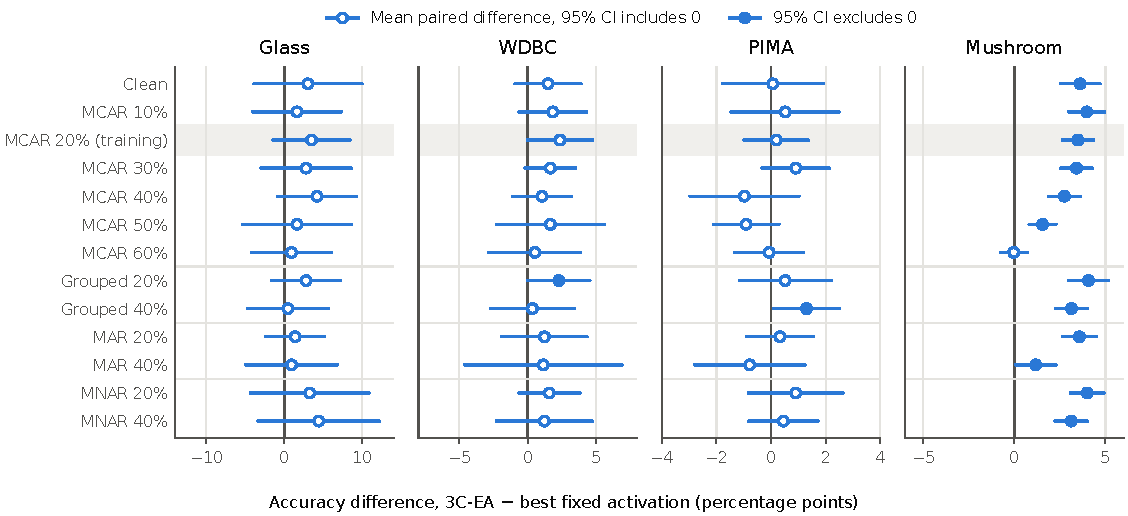
\includegraphics[width=\linewidth]{figures/fig_shift_differences.pdf}
\caption{Paired difference in test accuracy between 3C-EA and the best fixed activation under each test condition, for
models trained with 20\% MCAR missingness and then frozen. The shaded row is the matched reference condition. Points
are means over runs and bars are 95\% $t$-intervals of the paired difference; filled points mark intervals that
exclude zero. Horizontal axes differ between panels.}
\label{fig:shift-differences}
\end{figure}

\begin{table}[t]
\centering
\caption{Test accuracy of frozen models under missingness shift (mean $\pm$ standard deviation over runs). All models are trained with 20\% MCAR
missingness; the first row is the matched reference condition and the remaining rows are the twelve shifted
conditions. \emph{Fixed} is the best of ReLU (R), Swish (S), LeakyReLU (L) and ELU (E) for that condition, indicated
by the subscript. The entry with the higher mean of each pair is in bold. $^{*}$ and $^{**}$ denote $p<0.05$ and $p<0.01$ in a
two-sided Wilcoxon signed-rank test between 3C-EA and the best fixed activation. In Mushroom about 1\% of the entries
are missing in the source data and remain missing in every condition.}
\label{tab:shift}
\vspace{3pt}
\scriptsize
\setlength{\tabcolsep}{3pt}
\resizebox{\linewidth}{!}{% generated by: python -m telo_tabular.shift_table (do not edit by hand)
\begin{tabular}{lcccccccc}
\toprule
 & \multicolumn{2}{c}{Glass} & \multicolumn{2}{c}{WDBC} & \multicolumn{2}{c}{PIMA} & \multicolumn{2}{c}{Mushroom} \\
\cmidrule(lr){2-3} \cmidrule(lr){4-5} \cmidrule(lr){6-7} \cmidrule(lr){8-9}
Test condition & 3C-EA & Fixed & 3C-EA & Fixed & 3C-EA & Fixed & 3C-EA & Fixed \\
\midrule
MCAR 20\% (reference) & $\mathbf{0.530{\pm}0.051}$ & $0.495{\pm}0.070_{\text{E}}$ & $\mathbf{0.960{\pm}0.019}$ & $0.936{\pm}0.028_{\text{R}}$ & $\mathbf{0.733{\pm}0.026}$ & $0.731{\pm}0.035_{\text{E}}$ & $\mathbf{0.979{\pm}0.008}$ & $0.967{\pm}0.021_{\text{E}}^{\dagger}$ \\
\midrule
Clean (0\%) & $\mathbf{0.574{\pm}0.067}$ & $0.544{\pm}0.061_{\text{E}}$ & $\mathbf{0.961{\pm}0.030}$ & $0.946{\pm}0.021_{\text{E}}$ & $0.751{\pm}0.026$ & $0.751{\pm}0.043_{\text{E}}$ & $\mathbf{0.998{\pm}0.003}^{**}$ & $0.962{\pm}0.022_{\text{L}}$ \\
MCAR 10\% & $\mathbf{0.547{\pm}0.057}$ & $0.530{\pm}0.067_{\text{E}}$ & $\mathbf{0.959{\pm}0.023}$ & $0.940{\pm}0.026_{\text{E}}$ & $\mathbf{0.740{\pm}0.025}$ & $0.735{\pm}0.030_{\text{E}}$ & $\mathbf{0.993{\pm}0.004}^{**}$ & $0.953{\pm}0.020_{\text{L}}$ \\
MCAR 30\% & $\mathbf{0.514{\pm}0.046}$ & $0.486{\pm}0.086_{\text{E}}$ & $\mathbf{0.949{\pm}0.017}$ & $0.932{\pm}0.038_{\text{E}}$ & $\mathbf{0.735{\pm}0.028}$ & $0.726{\pm}0.029_{\text{E}}$ & $\mathbf{0.964{\pm}0.006}^{**}$ & $0.930{\pm}0.020_{\text{L}}$ \\
MCAR 40\% & $\mathbf{0.500{\pm}0.051}$ & $0.458{\pm}0.060_{\text{E}}$ & $\mathbf{0.942{\pm}0.015}$ & $0.932{\pm}0.027_{\text{E}}$ & $0.706{\pm}0.030$ & $\mathbf{0.716{\pm}0.019}_{\text{E}}$ & $\mathbf{0.937{\pm}0.008}^{**}$ & $0.910{\pm}0.022_{\text{L}}$ \\
MCAR 50\% & $\mathbf{0.493{\pm}0.066}$ & $0.477{\pm}0.078_{\text{E}}$ & $\mathbf{0.932{\pm}0.023}$ & $0.916{\pm}0.039_{\text{E}}$ & $0.696{\pm}0.022$ & $\mathbf{0.705{\pm}0.029}_{\text{E}}$ & $\mathbf{0.899{\pm}0.011}^{**}$ & $0.884{\pm}0.021_{\text{L}}$ \\
MCAR 60\% & $\mathbf{0.458{\pm}0.056}$ & $0.449{\pm}0.069_{\text{E}}$ & $\mathbf{0.911{\pm}0.026}$ & $0.906{\pm}0.043_{\text{E}}$ & $0.685{\pm}0.023$ & $\mathbf{0.686{\pm}0.028}_{\text{E}}$ & $0.848{\pm}0.024$ & $0.848{\pm}0.022_{\text{L}}$ \\
\addlinespace[2pt]
Grouped 20\% & $\mathbf{0.523{\pm}0.043}$ & $0.495{\pm}0.074_{\text{E}}$ & $\mathbf{0.955{\pm}0.020}$ & $0.932{\pm}0.032_{\text{E}}$ & $\mathbf{0.735{\pm}0.033}$ & $0.730{\pm}0.031_{\text{E}}$ & $\mathbf{0.979{\pm}0.006}^{**}$ & $0.938{\pm}0.023_{\text{L}}$ \\
Grouped 40\% & $\mathbf{0.458{\pm}0.072}$ & $0.453{\pm}0.051_{\text{E}}$ & $\mathbf{0.897{\pm}0.029}$ & $0.894{\pm}0.038_{\text{R}}$ & $\mathbf{0.726{\pm}0.025}$ & $0.713{\pm}0.032_{\text{E}}$ & $\mathbf{0.896{\pm}0.014}^{**}$ & $0.864{\pm}0.022_{\text{L}}$ \\
\addlinespace[2pt]
MAR 20\% & $\mathbf{0.526{\pm}0.044}$ & $0.512{\pm}0.033_{\text{E}}$ & $\mathbf{0.943{\pm}0.026}$ & $0.931{\pm}0.040_{\text{E}}$ & $\mathbf{0.712{\pm}0.025}$ & $0.708{\pm}0.038_{\text{E}}$ & $\mathbf{0.967{\pm}0.006}^{**}$ & $0.931{\pm}0.021_{\text{L}}$ \\
MAR 40\% & $\mathbf{0.470{\pm}0.059}$ & $0.460{\pm}0.065_{\text{E}}$ & $\mathbf{0.896{\pm}0.036}$ & $0.885{\pm}0.066_{\text{E}}$ & $0.690{\pm}0.022$ & $\mathbf{0.697{\pm}0.017}_{\text{E}}$ & $\mathbf{0.855{\pm}0.019}^{*}$ & $0.843{\pm}0.025_{\text{L}}$ \\
\addlinespace[2pt]
MNAR 20\% & $\mathbf{0.530{\pm}0.061}$ & $0.498{\pm}0.072_{\text{E}}$ & $\mathbf{0.952{\pm}0.013}$ & $0.936{\pm}0.032_{\text{E}}$ & $\mathbf{0.724{\pm}0.035}$ & $0.715{\pm}0.023_{\text{E}}$ & $\mathbf{0.983{\pm}0.006}^{**}$ & $0.943{\pm}0.019_{\text{L}}$ \\
MNAR 40\% & $\mathbf{0.498{\pm}0.072}$ & $0.453{\pm}0.091_{\text{E}}$ & $\mathbf{0.925{\pm}0.020}$ & $0.912{\pm}0.049_{\text{E}}$ & $\mathbf{0.703{\pm}0.029}$ & $0.698{\pm}0.023_{\text{E}}$ & $\mathbf{0.951{\pm}0.008}^{**}$ & $0.919{\pm}0.019_{\text{L}}$ \\
\bottomrule
\end{tabular}
}
\end{table}

\subsubsection{Results}
Figure~\ref{fig:shift-curves} shows the accuracy as the test MCAR rate moves away from the training rate,
Figure~\ref{fig:shift-differences} shows the paired difference to the best fixed activation under the reference and
the twelve shifted conditions, and Table~\ref{tab:shift} lists the corresponding accuracies.

\emph{The evolved functions do not depend on the training missingness being present.} When the test data contain no
injected missingness, the accuracy of 3C-EA is equal to or higher than under the reference condition on all four
datasets (for example 0.998 against 0.979 on Mushroom and 0.574 against 0.530 on Glass). As the test rate increases,
accuracy decreases gradually, with no abrupt failure at any rate or under any mechanism, although the confidence values
supplied to the network are those computed at the 20\% training rate.

\emph{The advantage over fixed activations is retained under shift on three of the four datasets.} On Mushroom, 3C-EA
is more accurate than the best fixed activation in eleven of the twelve shifted conditions, by 1.2 to 4.1 percentage
points; ten of these differences have $p<0.001$ and the remaining one, MAR 40\%, has $p=0.044$. In nine conditions
3C-EA is ahead in every one of the 20 runs. On WDBC and Glass the mean difference is positive in all twelve shifted
conditions (0.4 to 2.3 and 0.5 to 4.4 points, respectively), but with 10 runs and test sets of 114 and 43 records none
of these differences is significant ($p\ge 0.06$ and $p\ge 0.13$), so they should be read as a consistent direction
and not as individually established effects. On PIMA the two approaches are equivalent: the difference ranges from $-1.0$ to
$+1.3$ points and changes sign across conditions.

\emph{The advantage does not grow with the amount of shift.} On WDBC and Mushroom the difference is largest at or next
to the training rate and shrinks as the test rate increases; on Glass it varies between 1.6 and 4.2 points up to 50\%
without a clear trend. At 60\% MCAR the difference is at most 0.9 points on every dataset, and on Mushroom the two
methods coincide (0.848). Under the structured mechanisms the difference at 40\% is smaller than at 20\% in ten of the
twelve dataset--mechanism pairs; the exceptions are MNAR on Glass and grouped missingness on PIMA. This contrasts with
Figure~\ref{fig:performance}, where the models are evolved and trained separately at each missing rate and the gap
widens with the rate. Taken together, the two experiments suggest that the benefit of 3C-EA comes from adapting the
activation function to the missingness regime seen during evolution. That benefit carries over to moderately different
test conditions, but we find no evidence that an evolved function tolerates heavy unseen missingness better than a
fixed activation.

For completeness, we ran the same experiment on Sonar, the remaining complete dataset. There, 3C-EA is ahead in four of
the twelve shifted conditions and level or behind in eight, with differences between $-3.3$ and $+2.9$ points and none
significant
(test set of 42 records), in line with the Sonar results in Table~\ref{tab:mcar}, where no method is consistently
best.

Finally, these comparisons are made under the common training budget of \S\ref{sec:baselines}, which is identical for
all methods and is not tuned separately for each activation function.

\end{document}
